%
%%%%%%%%%%%%%%%%%%%%%%%%%%%%%%%%%%%%%%%%%%%%%%%%%%%%%%%%%%%%%%%%%%%%%%%%%%%%%%%%
\chapter{Theoretical background}\label{chap:1}
%%%%%%%%%%%%%%%%%%%%%%%%%%%%%%%%%%%%%%%%%%%%%%%%%%%%%%%%%%%%%%%%%%%%%%%%%%%%%%%%
%
%%%%%%%%%%%%%%%%%%%%%%%%%%%%%%%%%%%%%%%%%%%%%%%%%%%%%%%%%%%%%%%%%%%%%%%%%%%%%%%%
\section{Introduction}\label{sec:intro}
%%%%%%%%%%%%%%%%%%%%%%%%%%%%%%%%%%%%%%%%%%%%%%%%%%%%%%%%%%%%%%%%%%%%%%%%%%%%%%%%
%
Since the \todo{theoretical prediction?} of skyrmions in \todo{year?}
\todo{cite} and their experimental discovery in \todo{year} \todo{cite},
skyrmions have been extensively investigated both by theorists and
experimentalists \todo{some refs}. Skyrmions have caused a lot of excitement
mostly due to their promising properties that might qualify them as fast and
efficient memory. Three-dimensional non-perturbative classical Monte Carlo
methods developed recently~\cite{skyrmionlattice}, allow us to compute the full
finite temperature phase diagram and explore phase transitions. The goal of this
project was to implement the discretized lattice Hamiltonian introduced
in~\cite{skyrmionlattice} and basically reproduce the results discussed there.
In contrast to most previous work on Monte Carlo methods describing skyrmions,
we want to provide a detailed exposition of the algorithms and numerical
aspects. The report can serve as an ab initio step-by-step introduction on how
to write Monte Carlo methods and associated pitfalls or caveats based on a
concrete example. All code is publicly available on GitHub under
\todo{link} and we hope that it will be useful to others.

We introduce the model in \secref{sec:model} and briefly outline the general
idea of Monte Carlo methods on an abstract level. In \secref{sec:mctheory} we
introduce Monte Carlo techniques more formally and state some important
properties and results mostly without proofs. Moreover we discuss verification
strategies for Monte Carlo codes. \Secref{sec:code} contains the documentation
of our code as well as a user manual. Moreover, we provide reasoning for design
decisions. Physical results of the simulations are presented in
\secref{sec:results}. Finally, we conclude in \chapref{chap:3}.
%
%%%%%%%%%%%%%%%%%%%%%%%%%%%%%%%%%%%%%%%%%%%%%%%%%%%%%%%%%%%%%%%%%%%%%%%%%%%%%%%%
\section{The Spin Lattice Model}\label{sec:model}
%%%%%%%%%%%%%%%%%%%%%%%%%%%%%%%%%%%%%%%%%%%%%%%%%%%%%%%%%%%%%%%%%%%%%%%%%%%%%%%%
%
A common high-level way to think about magnetism in condensed matter is in terms
of complex collective behavior of spins, each of which is associated to a
magnetic moment. Astoundingly this simple model is quite powerful and allows for
an thorough explanation of a wide range of phenomena. Let us consider a
three-dimensional lattice with equidistant spacing in each direction. To each
lattice site we attach a spin, represented by an arbitrary element of the unit
sphere~$S^2$, see \figref{fig:lattice}. In the following we will often resort to
the two-dimensional model for illustration purposes, because it is easier to
draw on a two-dimensional surface. Each lattice sites typically represents a
nucleus, hence the whole lattice can be interpreted as a regular atomic
structure of a solid.

\begin{figure}
  \centering
  \begin{tikzpicture}
    \latticeinter{4}
    \begin{scope}[xshift=8cm,yshift=1cm]
      \lattice{4}
    \end{scope}
  \end{tikzpicture}%
  \caption{On the left side we show a two-dimensional spin lattice. Each lattice
  site carries a magnetic moment or spin, represented by an arrow of unit
  length, \ie{}, in the two-dimensional picture, by an element of~$S^1$. The
  neighbors of a lattice site are the ones above, below, left and right in
  two-dimensional case. The blue squares are the neighbors of the red circle.
  The three-dimensional picture on the right side becomes unclear in a
  two-dimensional drawing rather quickly. Note that the magnetic moments are now
  also three-dimensional, \ie{} elements of the two-dimensional unit
  sphere~$S^2$. In the three-dimensional a lattice site can have six neighbors.}
\label{fig:lattice}
\end{figure}

We work with a simple cubic lattice
%
\begin{equation}
  \Sigma := \numlist{1}{N_x} \times \numlist{1}{N_y} \times
  \numlist{1}{N_z} \subset \bN^3 \subset \bR^3\:,
\end{equation}
%
where we interpret~$(i,j,k) \in \Sigma$ as~$i \hx + j \hy + k \hz
\in \bR^3$. Note that we can translate the whole lattice by arbitrary integer
linear combinations of the standard basis vectors, thus starting at~$(1,1,1)$
does not have any physical meaning. It merely translates nicely to the numerical
implementation in any~$1$-indexed programming language. Here,~$\hx,
\hy, \hz$ are the standard basis vectors of~$\bR^3$. At each point~$\r
\in \Sigma$ we attach a spin~$\S_{\r} \in S^2$, which yields an overall
configuration space~$\Pi := \prod_{\r \in \Sigma} S^2$.  Each element of~$\Pi$
consists of~$\abs{\Sigma}=N_x N_y N_z$ spins, \ie{} elements of~$S^2$, thus
describes one possible spin configuration of the whole lattice. We refer to the
specific spin at position~$\r \in \Sigma$ with~$\S_{\r} \in S^2$.  Note that we
only discretize the positions of the spins, but not explicitly their directions.
In any real implementation they are of course discretized by the finite count of
floating point numbers. This mirrors the naturally discretized crystal structure
of solids.

% While the microscopic field within the solid varies greatly over distances on
% the order of the lattice spacing, from far away those microscopic fluctuations
% smear out and we observe an averaged macroscopic field. For example, when we
% choose each spin uniformly at random, as we did in \figref{fig:lattice}, one
% expects the overall macroscopic field to be zero for a sufficiently large
% system.

The goal of our simulation is to find a state~$\pi \in \Pi$ that minimizes the
energy of the system for given parameters. You might notice that we have not
defined a notion of energy yet nor explicitly listed the free parameters of such
a spin lattice. Apparently any physical measure of energy must be based on
interactions between the spins within the system or also with external fields.
Let us elaborate on some possible interactions. Each of them comes with a
constant that can be interpreted as a weight, \ie{} how much the respective
interaction contributes to the action with respect to the others. Those
constants are parameters of the system.

\subsection{Interactions}

\subsubsection{Ferromagnetic/direct exchange}

The most obvious interaction is the \newterm{ferromagnetic} or \newterm{direct}
exchange.  Pictorially speaking, it favors constellations where spins that are
close to each other point into the same direction. A system only interacting
this way will end up in a state where all spins are parallel to each other. The
measure for parallelism of two neighboring spins~$\S_{\r_1}, \S_{\r_2} \in S^2$
can be expressed as~$- \S_{\r_1} \cdot \S_{\r_2} = - \norm{\S_{\r_1}}
\norm{\S_{\r_2}} \cos(\alpha)$, where~$\alpha$ is the angle between~$\S_{\r_1}$
and~$\S_{\r_2}$. The minus sign ensures that the energy of two parallel spins is
actually smaller than the energy of two perpendicular or even antiparallel ones.
In the continuum, the direct exchange term consists of a gradient, which is a
local quantity, \ie{} the gradient at a point only depends on an arbitrarily
small neighborhood of the point. Thus we will always consider the ferromagnetic
exchange to be \newterm{local} or \newterm{short ranged} in the sense that it
only contributes for adjacent lattice sites and we can thus hide the distance in
an overall constant, see \todo{figref}.

\subsubsection{Interaction with an external field}

Another important exchange term describes the interaction of the system with an
\newterm{external magnetic field}. Clearly, every spin tries to align with an
external field~$\B$, which we express mathematically via~$-\B \cdot \S$ for
every spin~$\S$ on the lattice. It can be misleading to use terms such as
\newterm{non-local} or \newterm{long ranged} for this exchange, since it is not
an interaction between two or more spins within the system, but affects each
lattice site independently in the same way. Naturally, for the external
field,~$\B$ itself is the parameter of the interaction.

\subsubsection{Dipole-dipole interaction}

These two are the most commonly encountered exchange terms. The
\newterm{dipole-dipole interaction} is somewhat more complex, but also weaker.
For two spins~$\S_{\r_1}, \S_{\r_2} \in S^2$, it is given by
%
\begin{equation}
  - {\norm{\r}^{-3}} (3 (\S_{\r_1} \cdot \hat{\r})
  (\S_{\r_2} \cdot \hat{\r}) - \S_{\r_1} \cdot \S_{\r_2})\:,
\end{equation}
%
where~$\r = \r_2 - \r_1$ and~$\hat{\r} = \r / \norm{\r}$ points from the
location of the first spin to the location of the second one. The dipole-dipole
interaction depends on the distance between the two lattice sites as well as the
orientation of the two spins not only relative to each other, but also to the
line connecting them. Moreover, the explicit dependence on the relative position
already indicates that the dipole-dipole interaction is relevant for each pair
of spin in the system, it is a long ranged interaction. In a system of~$N^3$
lattice sites, the number of pairs scales like~$N^6$. Hence, most simulations do
not take the dipole-dipole exchange into account purely due to limited
computational resources. The same holds true for our example.

\subsubsection{Dzyaloshinskii-Moriya exchange}

In this work we are interested in chiral magnets, certain crystals that lack
inversion symmetry, \eg{} MnSi. This gives rise to the so called \newterm{weak
Dzyaloshinskii-Moriya} (DM) coupling. In the continuum it is described by a term
proportional to~$-\S(\r) \cdot (\nabla \times \S(\r))$. Just like the gradient,
the curl of a vector field is a local property, thus the DM exchange only
contributes for adjacent lattice sites. The discretized version for two
spins~$\S_{\r_1}, \S_{\r_2} \in S^2$ at neighboring positions~$\r_1, \r_2 \in
\Sigma$ reads~$- (\S_{\r_1} \times \S_{\r_2}) \cdot (\r_2 - \r_1)$.  Since the
cross product is zero for parallel vectors and maximal for perpendicular vector,
the DM coupling acts to some extent against the ferromagnetic interaction and
favors constellations where adjacent spins are perpendicular to each other.

\todo{Why is ferromagnetic exchange always canonically local (neighboring only)
and dipole dipole interaction would be between all pairs?}

\subsection{The Hamiltonian}

Let us now combine the FM and DM interaction as well as an external magnetic
field to compute the energy for the lattice~$\Sigma$. To this end we add up the
contributions from each spin and for each interaction. For instance, the
external field exchange term simply becomes
%
\begin{equation}\label{Bsum}
  -\sum_{\r \in \Sigma} \S_{\r} \cdot \B\:.
\end{equation}
%

Adding up the terms for the FM interaction with all direct neighbors naively as
in
%
\begin{equation}\label{FMsumnaive}
  -\sum_{\r \in \Sigma} \S_{\r} \cdot (\S_{\r + \hx} + \S_{\r - \hx} +
    \S_{\r + \hy} + \S_{\r - \hx} + \S_{\r + \hz} + \S_{\r - \hz})\:,
\end{equation}
%
poses two problems. First, apparently in this fashion we count the interaction
between some pairs of spins multiple times. If~$\Sigma$ was an infinite grid,
\ie{}~$\Sigma=\bZ^3$, we would count every pair exactly twice and could simply
divide the above expression by two. However,~$\Sigma$ is finite, which leads us
to the second, more subtle, issue. Not every lattice site has a neighbor in each
direction~$\hx, \hy, \hz$. Consider the spin in the lower right corner of a
lattice in figure \todo{figref}. The sum in our first naive expression for the
FM interaction~\eqref{FMsumnaive} suggests that we need its right and lower
neighbor, which apparently do not exist. As a consequence, we need to define
some \newterm{boundary conditions}. There are several ways to do this and a
plausible treatment of boundaries is a central aspect of many different areas in
scientific computing. It is important to realize that this is not simply an
implementation nuisance that we can get rid off by any means that make the code
work. Various boundary conditions represent different physical systems and
significantly alter the results of a simulation.

In many cases the desired simulation volume is an infinite space such
as~$\bR^3$. A common choice to get as close as possible on our inherently finite
computers is to introduce \newterm{periodic boundary conditions}. We
approximate~$\bR^3$ by a finite box of volume~$L^3$ for~$L\in \bRp$ and simply
replicate that box infinitely many times to fill the whole space, see
\figref{fig:periodic} for a two-dimensional illustration. In practice, we will
access the lattice sites by indexing a three-dimensional array with
indices~$(i,j,k)\in\Sigma$. Whenever the algorithm tries to index out of bounds,
\eg{}~$j=N_y + 1$, we simply use~$j=1$ again. For~$i=0$ we use~$i=N_x$,
for~$k=N_z+2$ we use~$k=2$ and so on. In general, this behavior can be achieved
by always working with the indices
%
\begin{equation}\label{periodicindices}
  ((i-1 \mod N_x) + 1, (j-1 \mod N_y) + 1, (k-1 \mod N_z) + 1) \in \Sigma
\end{equation}
%
whenever the algorithm requests data at position~$(i,j,k) \in \bZ^3$. By
construction, those new indices always lie in~$\Sigma$. We can now
unproblematically include spins at officially non-existing positions in our
mathematical expressions, implicitly assuming that those are being wrapped
around periodically to positions within the lattice. In our first simulations,
we will employ periodic boundary conditions in all three directions
using~\eqref{periodicindices}. For other scenarios we opened up the boundaries
in one direction. \newterm{Open boundaries} can be realized by setting~$\S_\r =
0$ for all~$\r \in \bZ^3 \setminus \Sigma$. While periodic boundary conditions
try to mimic an infinite space, open boundaries clearly represent a finite
extension of the simulation volume in the respective direction. We will come
back to open boundaries later. This solves the second issue.

\begin{figure}
  \centering
  \begin{tikzpicture}
    \periodic{}
  \end{tikzpicture}
  \caption{We illustrate periodic boundary conditions for a
  two-dimensional~$4\times4$ grid. The actually implemented simulation value is
  given by the shaded square in the middle. This square is copied over and over
  again in all directions as indicated by the surrounding lattice sites. Note
  how the four boundaries of the square keep their orientation throughout that
  copying procedure. While it appears like we have filled an infinite space, all
  red squares are identified, because they are represented internally by only
  one lattice site in the central square. The same holds true for the green
  pentagons of course. If our code needs the value of the right neighbor of the
  green pentagon in the central square for example, we can instead pick the
  right neighbor of \emph{any} green pentagon. One of those will always lie in
  the center square again and thus be available in memory.}
\label{fig:periodic}
\end{figure}

Now that we have a well defined boundary behavior, we can also tackle the first
problem of counting interactions multiple times. Indeed we could now divide the
whole expression by~$2$, or, even simpler, write it as
%
\begin{equation}\label{FMsum}
  -\sum_{\r \in \Sigma} \S_{\r} \cdot
    (\S_{\r + \hx} + \S_{\r + \hy} + \S_{\r + \hz})\:.
\end{equation}
%
It is worth convincing oneself that in this expression with periodic boundary
conditions every pair of neighboring lattice sites is included exactly once.

Finally, the DM term for the whole lattice is
%
\begin{equation}\label{DMsum}
  -\sum_{\r \in \Sigma} ((\S_{\r} \times \S_{\r + \hx}) \cdot \hx +
    (\S_{\r} \times \S_{\r + \hy}) \cdot \hy +
    (\S_{\r} \times \S_{\r + \hz}) \cdot \hz)\:.
\end{equation}
%
Everything we discussed about boundary conditions for the FM exchange also holds
true for the DM interaction.

Ultimately adding up all interactions~\eqref{Bsum},~\eqref{FMsum}
and~\eqref{DMsum}, we obtain the Hamiltonian, \ie{} the energy of the system in
a given configuration~$\pi \in \Pi$
%
\begin{align}\label{hamiltonian}
  H(\pi) = &-\sum_{\r \in \Sigma}\biggl(\S_{\r} \cdot \B +
      J \S_{\r} \cdot (\S_{\r+\hx} + \S_{\r+\hy} + \S_{\r+\hz}) \\
      &+ K (\S_{\r} \times \S_{\r+\hx} \cdot \hx +
            \S_{\r} \times \S_{\r+\hy} \cdot \hy +
            \S_{\r} \times \S_{\r+\hz} \cdot \hz)\biggr)\:.
\end{align}
%
The parameters~$J$,~$K$ and~$\B$ are sometimes used synonymously for the
ferromagnetic, the Dzyaloshinskii-Moriya and the external field interaction
terms. As we will see in the simulation results in \chapref{chap:3}, the
physical behavior of the system strongly depends on these freely adjustable
parameters. For a given set of parameters and at zero temperature we typically
define the physical configuration to be the
%
\begin{equation}\label{objective}
  \argmin_{\pi \in \Pi} H(\pi)\:.
\end{equation}

\subsubsection{Finite size effects}

\todo{just include extra terms of finite size effects, note that it is not
really a next neighbor interaction, but just a correction, draw picture, make
distinction between boundary effects and finite size effects clearer: rewrite
discussion about trying to mimic infinite space and instead say that boundary
can do weird things otherwise}

\subsection{A note on parameter values}

Recall that there is a great conflict of interest between the FM and
the DM interactions. While the FM term in the Hamiltonian is minimal when all
spins are parallel to each other, the DM term favors a configuration where
neighboring spins are orthogonal. The specific compromise between those effects
depends mostly on their respective strength~$J$ and~$K$. In reality the direct
interaction~$J$ is much stronger and one typically encounters helical
structures with long modulation periods, see \todo{figref}. For example in MnSi
the spins wind around a given modulation axis only once per roughly~$40$ lattice
spacings. By tuning the ratio~$J/K$ we can set the periodicity. For a
periodicity of~$N$ lattice sites, we have to set~$J/K$ to~$\tan(2\pi / N)$. In
all our simulations we chose~$J=1$ and~$K=\tan(2\pi / 10)$. Moreover, we choose
the external magnetic field to point in the~$\hz$ direction~$\B=(0,0,B)$.

We can fix one of the parameters, in this case~$J$, arbitrarily and then work in
abstract lattice units. A computer can only deal with dimensionless numbers and
in numerical simulations one often makes some convenient, but arbitrary choices.
It is then sometimes quite difficult to translate the results to physically
meaningful values.

The alert reader might have realized that so far our model does not contain any
thermal energy. When talking about magnetism temperature typically has a strong
influence on the physical properties of various materials. However, given the
challenge to incorporate a temperature dependent term into the Hamiltonian that
accounts for the thermal energy, we quickly realize that it is not that simple.
Any additive term that depends solely on the temperature will not have any
effect on~\eqref{objective}. On the other hand there is no physical reason for
complex interaction terms that actually yield different configurations for
different temperatures. Our intuition tells us that thermal energy is
intrinsically of dynamic nature, thus cannot be captured in a single static spin
configuration. In fact we will account for temperature in the optimization
algorithm itself and clearly see the dynamic nature of it in \secref{mctheory}.

\subsection{Summary}

In this section we have set up our model, which we will briefly summarize here.
We work on the lattice
%
\begin{equation}
  \Sigma := \numlist{1}{N_x} \times \numlist{1}{N_y} \times
  \numlist{1}{N_z} \subset \bN^3 \subset \bR^3\:
\end{equation}
%
and attach a spin~$\S_{\r} \in S^2$ to each lattice site~$\r \in \Sigma$. This
yields the configuration space
%
\begin{equation}
  \Pi := \prod_{\r \in \Sigma} S^2\:.
\end{equation}
%
On~$\Pi$ we define the Hamiltonian~\eqref{hamiltonian} where we implement
periodic (and sometimes partially open) boundary conditions. We fix the
parameters~$J=1$ and~$K=\tan(2\pi / 10)$ of the FM and DM interaction, which
leaves us only with the magnetic field in the~$\hz$ direction~$B$. In the next
section we will introduce the temperature as a second parameter. Very
roughly speaking, for given values of~$B$ and~$T$ we then seek to
minimize~$H(\pi)$. The minimizing configuration is considered to be the physical
one.


%
%%%%%%%%%%%%%%%%%%%%%%%%%%%%%%%%%%%%%%%%%%%%%%%%%%%%%%%%%%%%%%%%%%%%%%%%%%%%%%%%
\section{Monte Carlo Methods}\label{sec:mctheory}
%%%%%%%%%%%%%%%%%%%%%%%%%%%%%%%%%%%%%%%%%%%%%%%%%%%%%%%%%%%%%%%%%%%%%%%%%%%%%%%%
%
Now that we have clearly stated the model, let us dive into the numerical
methods. Monte Carlo methods is a very broad term that is generally used for
numerical algorithms that are based on some sort of repeated random sampling. It
is hard to formulate a more specific feature that all Monte Carlo algorithms
have in common. Most often, Monte Carlo techniques are used for optimization,
integration or sampling probability distributions. Since we are interested in
optimization, we will restrict our discussion of Monte Carlo methods entirely to
this subfield. Before we describe our algorithm of choice in detail, we have to
issue a warning. While Monte Carlo methods are generally easy to implement and
can be applied blindly to virtually any problem, they are almost always
hopelessly inferior to specialized optimization techniques in terms of accuracy
and efficiency. They should be the last resort after everything else has failed.

In a typical optimization problem we seek to find the minimum of a real-valued
function~$f$ over some subset of its domain~$\Omega \subset \bR^n$. Depending
on~$f$ and~$\Omega$ this can be anything from trivial to practically infeasible.
This gives rise to numerous possible classification schemes. Let us briefly
mention two important properties. First, we distinguish optimization techniques
by whether they use Hessians, gradients or only function values. Apparently the
degree of differentiability of the objective function~$f$ plays a crucial role.
If~$f$ is sufficiently smooth and we have access to gradients (and Hessians)
either analytically or numerically, we can build a first order (second order)
approximation to the function at a given point~$x \in \Omega$. This leads to so
called local methods, where we have to specify a start point, approximate the
function around this point, proceed in the downward direction and repeat the
procedure. Numerous gradient-descent and (Quasi-)Newton methods fall into that
category of iterative methods. The convergence rate and also the complexity
depend on how much information we have about the derivatives of the function,
but most iterative methods are guaranteed to converge to a minimum for
sufficiently well behaved functions and wisely chosen parameters.

The major caveat with local methods is precisely that they find \emph{a}
minimum, but potentially not \emph{the} minimum. If a function has several local
minima, depending on the start point, we might end up in any of them and
potentially overlook a global minimum somewhere else hidden to our descent
method by a barrier. In this case we could either still employ iterative methods
with multiple starting points and hope that one of them guides us to the global
minimum, or switch to heuristics. Heuristics are not mathematically guaranteed
to find the solution, in fact very little can be proven about how well
heuristics will do in general. However, they often prove very useful, especially
if we do not have an applicable finitely terminating or at least provably
convergent iterative algorithm, see \figref{fig:samplefuncs}. Interestingly,
many heuristics have been inspired by natural processes like the genetic
algorithms, bee or ant colony optimization, evolutionary algorithms or simulated
annealing.

\begin{figure}
  \centering
  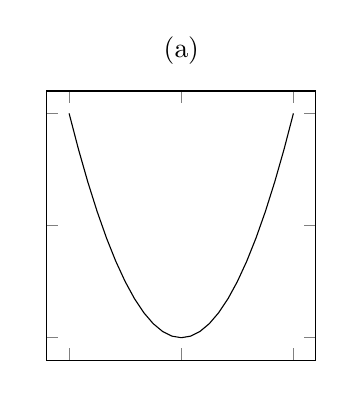
\begin{tikzpicture}
    \begin{axis}[
        width=5cm,
        height=5cm,
        title={(a)},
        % label style={font=\small},
        % xlabel={$x$},
        % ylabel={$f(x)$},
        yticklabels={,,},
        xticklabels={,,},
      ]
      \addplot[domain=-1:1] {x^2};
    \end{axis}
  \end{tikzpicture}%
  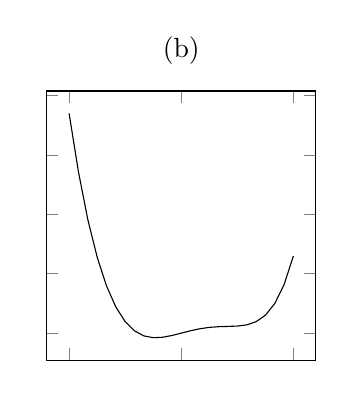
\begin{tikzpicture}
    \begin{axis}[
        width=5cm,
        height=5cm,
        title={(b)},
        % label style={font=\small},
        % xlabel={$x$},
        % ylabel={$f(x)$},
        yticklabels={,,},
        xticklabels={,,},
      ]
      \addplot[domain=-1:1] {x - 5*x^3 + 5*x^4 + 1.6*x^5};
    \end{axis}
  \end{tikzpicture}%
  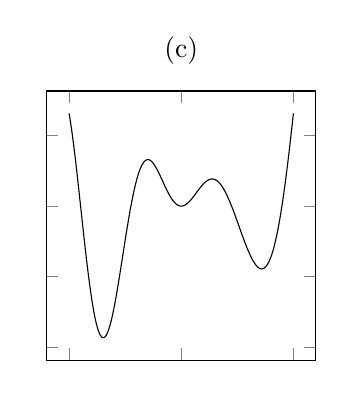
\begin{tikzpicture}
    \begin{axis}[
        width=5cm,
        height=5cm,
        title={(c)},
        % label style={font=\small},
        % xlabel={$x$},
        % ylabel={$f(x)$},
        yticklabels={,,},
        xticklabels={,,},
      ]
      \addplot[domain=-1:1, samples=1000] {sin(deg(7*x))*(x^4 - x^2 + x)};
    \end{axis}
  \end{tikzpicture}%
  \begin{tikzpicture}
    \begin{axis}[
        width=5cm,
        height=5cm,
        title={(d)},
        % label style={font=\small},
        % xlabel={$x$},
        % ylabel={$f(x)$},
        yticklabels={,,},
        xticklabels={,,},
      ]
      \addplot[solid, mark=none]
        table[x expr=\coordindex+1, y index=0] {plots/energy_landscape.csv};
    \end{axis}
  \end{tikzpicture}%
  \caption{Convex functions like the one shown in (a) can be minimized extremely
  efficiently even on high-dimensional domains. While the second example (b) is
  not convex anymore, it is smooth and has a unique minimum. Therefore local
  iterative methods will do an excellent job and converge quickly to the
  minimum. Function (c) is still smooth, but has several minima. Depending on
  where we position the starting point, iterative gradient methods might get
  stuck in one of the two local minima on the right and not find the global
  minimum on the left. The fourth function (d) is not even once differentiable
  and has numerous minima. We can only use heuristics and hope to get close to
  the true minimum.}
\label{fig:samplefuncs}
\end{figure}

The domain of our optimization problem is a~$2 N_x N_y N_z$-dimensional space.
Even for relatively small lattices optimization in such a high-dimensional space
is generically hard. Unfortunately, it appears completely hopeless to compute
the gradient or even Hessian of the Hamiltonian~\eqref{hamiltonian}
analytically. Moreover, it is hard to develop intuition about how the energy
landscape looks like, not only because we can barely visualize anything in more
than three dimensions. It appears certain, however, that it will include a vast
number of local minima. All of this is bad news for efficient iterative methods
and we have to fall back to heuristics. Our only option is to sample the search
space preferably in a smart and structured way and hope to capture the minimum
within reasonable computation time. This is precisely what Monte Carlo methods
do. They consist of a sampling strategy that involves some randomness.
Obviously, this sounds horrifically inefficient, which it is. Now we understand
why Monte Carlo techniques should only be considered once everything else failed
or proved intractable.

For our use case we implemented \newterm{simulated annealing}. The name already
hints towards thermodynamic processes, which we already identified as a key
feature of our system, but were not yet able to bake it into our model. Clearly
any real material at finite temperature is not completely static, \ie{} stuck in
a fixed state~$\pi \in \Pi$, but it is constantly subject to thermal
fluctuations. Apparently our current objective, finding a unique global minimum
of the Hamiltonian for given parameters, is insufficient. Simulated annealing is
designed to mimic real world systems at finite temperature and will take care of
thermal fluctuations. That implies that we will not seek to find a single best
state~$\pi \in \Pi$ anymore, but consider the physical state to be a thermal
average of several configurations. To fully understand and appreciate simulated
annealing, we need some basic concepts from statistical physics.

In macroscopic complex many body systems such as gases or condensed matter at
finite temperature, we are often not interested in every single detail of that
system at a given moment in time.  For example, we do not want to know the
position and velocity as well as rotational and vibrational modes of each single
molecule in a piston. Sensible observables are typically some sort of
macroscopic averages like the volume, temperature or pressure of the gas. For a
solid we might be interested in its specific heat, conductivity or
susceptibility. Of course, there is a sound and rigorous way to define those
averages.

Instead of working with the complete microstates, in our case the elements
of~$\Pi$, directly, we only talk about the probability~$P_{\pi}(T)$ that the
system is in a certain state~$\pi \in \Pi$ at temperature~$T$. To this end we
imagine a large ensemble of replicas of the system and observe them all at the
same time. Starting from the assumption that in a closed system in equilibrium
each microstate~$\pi$ is equally likely, we can derive the so called canonical
ensemble which states that for a non-closed system in equilibrium at finite
temperature, \eg{} via contact to a large heat bath, we have
%
\begin{equation}\label{boltzmann}
  P_{\pi}(T) = \frac{\exp \left(- \frac{H(\pi)}{k_B T}\right)}
  {\sum_{\pi \in \Pi} \exp \left(- \frac{H(\pi)}{k_B T}\right)}\:.
\end{equation}
%
This is also referred to as the \newterm{equilibrium Boltzmann distribution}.
The normalizing factor in~\eqref{boltzmann}~$Z := \exp(-\beta H(\pi))$ is called
partition function. Here we introduced the common shortcut~$\beta := {(k_B
T)}^{-1}$, where~$k_B$ is the Boltzmann constant and~$T$ is the temperature of
the system. The equilibrium Boltzmann distribution tells us that configurations
with lower energy are exponentially more likely than configurations with a high
energy. Moreover, this effect is most pronounced at low temperatures. If~$T$ is
large, states with higher energy still occurr with a decent probability compared
to the minimizing state. On the other hand for~$T \to 0$ basically only the
state with minimal energy has a non-zero probability. Both facts completely
match our intuition. At high temperatures, thermal fluctuations are large and
the system can visit many different micro states. At zero temperature we expect
the system to settle in the ground state.

In a probabilistic description of states the energy or magnetization of one
single specific configuration looses its significance. Instead we transition to
expectations values of observables. For an observable~$\map{\cO}{\Pi}{\bR}$ we
compute the so called \newterm{thermal average}
%
\begin{equation}
  \avg{\cO} := \frac{1}{Z} \sum_{\pi \in \Pi} \cO(\pi) \exp(- \beta H(\pi))\:,
\end{equation}
%
hence we average over all states weighted by their probability at a given
temperature. One question immediately poses itself: How could be possibly
compute this high-dimensional integral?

\todo{clarify above that we could have finitely many states, but also a
continuum and then carry the sum/integral+measure, distribution thing through
(maybe example that ising would be finite, here it is infinite)}

\todo{should I actually start with integration instead of optimization for monte
carlo? if not, at least mention up front that the pure optimization thing is not
what we are going to do. It's more a combination in some sense}

\todo{the way we are sampling our space needs to contain detailed balance and
ergodicity. But why? I think that comes next and once we posed them, we
conclude that metropolis hastings might be a good idea}

\todo{draw a picture when we try to integrate a steep exponential we should
sample the ``lower energy'' boundary more often}

\begin{figure}
  \centering
  \begin{tikzpicture}
    \latticeselect{5}
    \begin{scope}[xshift=5.5cm]
      \latticeinter{5}
    \end{scope}
    \begin{scope}[xshift=11cm]
      \latticeinternn{5}
    \end{scope}
  \end{tikzpicture}%
  \caption{\todo{explain what neighbors are, what next neighbor interaction is,
  etc.}}
\label{fig:interact}
\end{figure}
